%	pictures for the introduction:
%	- map of Daghestan with locations
%	- picture of Sanzhi
%	- picture of Druzhba
%	- picture of Gadzhimurad with books
%	- picture of me while talking to Sanijat
%	CHECK Iwona's pics



\chapter{Introduction}
\label{cpt:Introduction}

%%%%%%%%%%%%%%%%%%%%%%%%%%%%%%%%%%%%%%%%%%%%%%%%%%%%%%%%%%%%%%%%%%%%%%%%%%%%%%%%

\section{The Sanzhi community and the Sanzhi language}
\label{sec:The Sanzhi community and the Sanzhi language}

Sanzhi Dargwa is an East Caucasian (i.e. Nakh-Daghestanian) language from the Dargwa (or Dargi) subbranch and belongs to the South Dargwa varieties. In the literature, there is no unique terminology referring to Dargwa languages, dialects or peoples, but several terms exist: Dargwa, Dargva, Dargi, or Darginskiy. For reasons of uniformity and unambiguousness I restrict myself to the label and the graphic representation \textit{Dargwa} and will not use the other terms. Sanzhi Dargwa is spoken by approximately 250 speakers and is heavily endangered. The self-designation of the Sanzhi people is \tit{sunglan-te} (Sanzhi.person\tsc{-pl}) and the language is called \tit{sunglan ʁaj} (lit. Sanzhi.person language).

More than 40 years ago, all Sanzhi speakers left the village of Sanzhi, their village of origin, in the Caucasian Mountains. Sanzhi is located in the Dakhadayevskiy rayon in central Dagestan (today part of the Russian Federation), which is predominantly inhabited by speakers of Dargwa languages.

The village of Sanzhi is located on the sunny side of the Ulluchay river valley, at an altitude of about 1,500 meters (\reffig{fig:Map 2}). The closest neighboring villages are Itsari, Shari, Khuduts, Ashty, and Amukh. The distance from Makhachkala is around 200 kilometers, from the regional center of the Dakhadayevskiy rayon, Urkarakh, it is 66 kilometers, and from Derbent around 150 kilometers. There is no direct road to Sanzhi. In order to reach the village, people go to Itsari by car or minibus and then walk around six kilometers until they reach Sanzhi. Currently, the Sanzhi territory is part of the nature park Itsari.

The village consists of approximately 30 houses, which are in very poor condition and not inhabited anymore (\reffig{fig:Sanzhi 1}, \reffig{fig:Sanzhi 2}, \reffig{fig:Sanzhi 3}). The only house with a roof that is relatively well kept is the former school building. Sanzhi people regularly go to Sanzhi in the summer to spend a few days fishing, berry picking, and doing other activities in their former village. The village is surrounded by terrace fields that have been used for centuries to grow crops such as rye, wheat, barley, oats, and in the recent past also carrots, radishes, potatoes, and others. The traditional occupations of the Sanzhi people were farming and breeding, in particular sheep breeding. Not far from the village, ancient rock paintings can be found that, according to the Sanzhi people, have been the subject of investigation by several researchers from Russia. Unfortunately, I was not able to find literature on the paintings or the research expeditions.

\begin{figure}
	\caption{The village of Sanzhi (courtesy of Gadzhimurad Gadzhimuradov)}
	\label{fig:Sanzhi 1}
	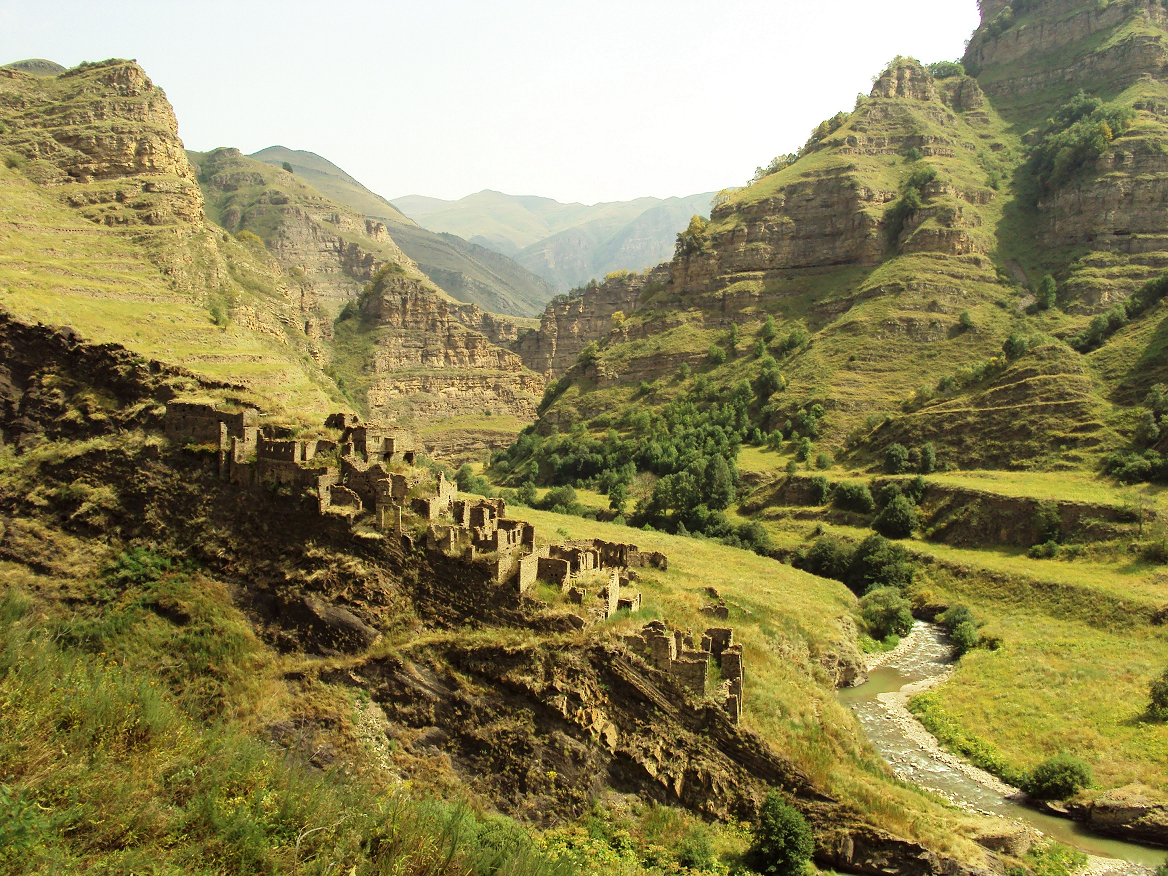
\includegraphics[scale=0.5, angle =90]{figures/Sanzhi_1.png}
\end{figure}

\begin{figure}
	\caption{The village of Sanzhi in 2013 (courtesy of Iwona Kaliszewska)}
	\label{fig:Sanzhi 2}
	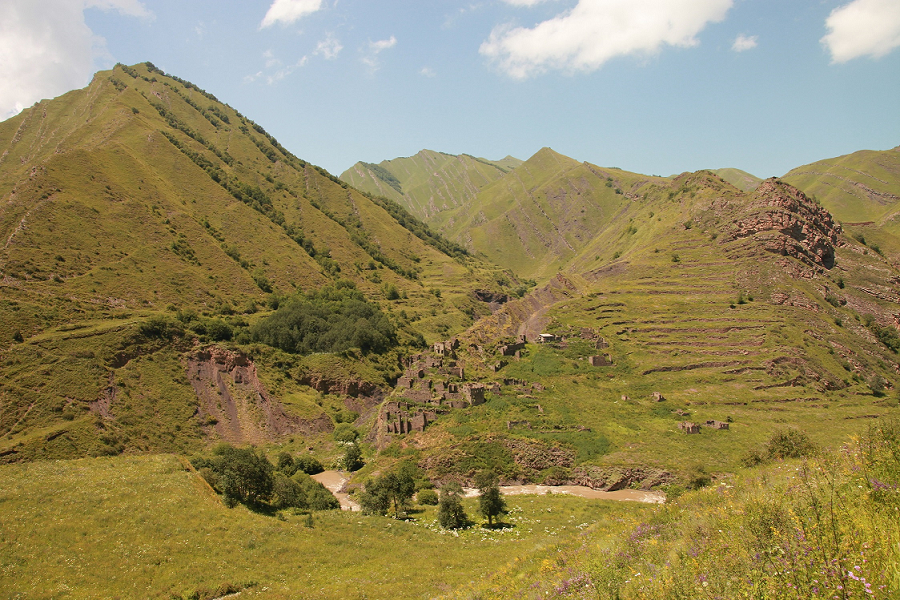
\includegraphics[scale=0.5]{figures/Sanzhi_2.png}
\end{figure}

\begin{figure}
	\caption{An old picture of Sanzhi, around 1957 (courtesy of the Sanzhi community)}
	\label{fig:Sanzhi 3}
	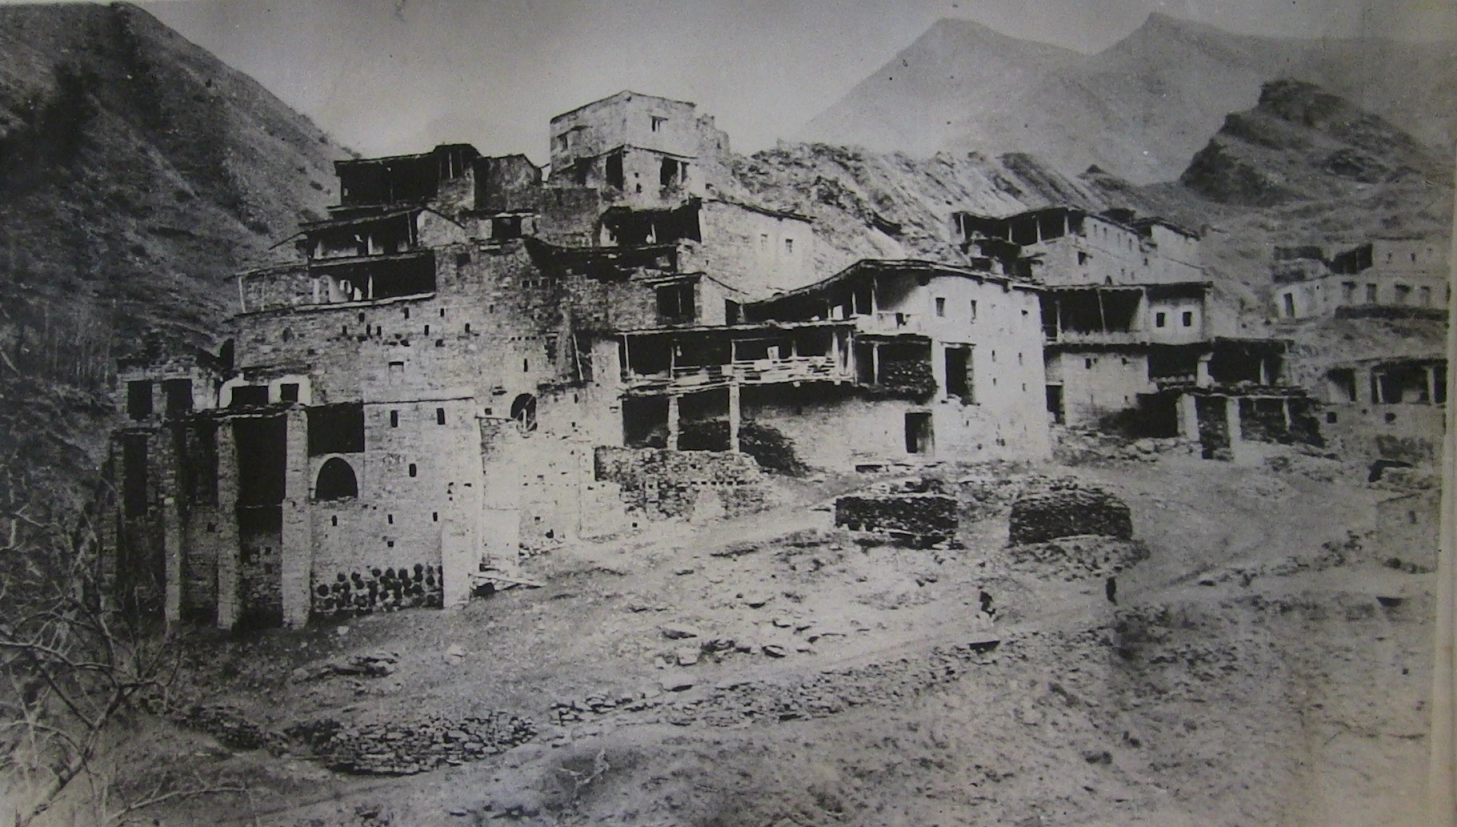
\includegraphics[scale=0.3]{figures/Sanzhi_3.png}
\end{figure}




From 1968 onwards, within a relatively short time span, all Sanzhi people moved to the lowlands to ethnically and linguistically mixed settlements. The major reason for the resettlement was the difficult life in the mountains. There was and still is no road leading to Sanzhi, and also no electricity. From grade five on, children had to walk by foot to the school in Itsari every day and under all weather conditions.

Today, the majority of Sanzhi speakers live in the village of Druzhba in the Daghestanian lowlands (Kayakentskiy Rayon) (\reffig{fig:Druzhba}) and to a lesser extent in other settlements in Daghestan and other parts of Russia. Druzhba is an ethnically and linguistically heterogeneous settlement with speakers of other South Dargwa varieties, other East Caucasian languages such as Tabasaran, Agul, Lezgian, and Lak, and also a very few Kumyk (Turkic) and Russian speakers. In Druzhba, people make a living by working in the local vineyards that used to be a collective farm. Many inhabitants, especially men, go to other parts of Russia to work there and support their families back home. A map of Daghestan with Sanzhi and Druzhba is given in \reffig{fig:Map 2}.

\begin{figure}
	\caption{The village of Druzhba in the winter of 2014 (picture by Diana Forker)}
	\label{fig:Druzhba}
	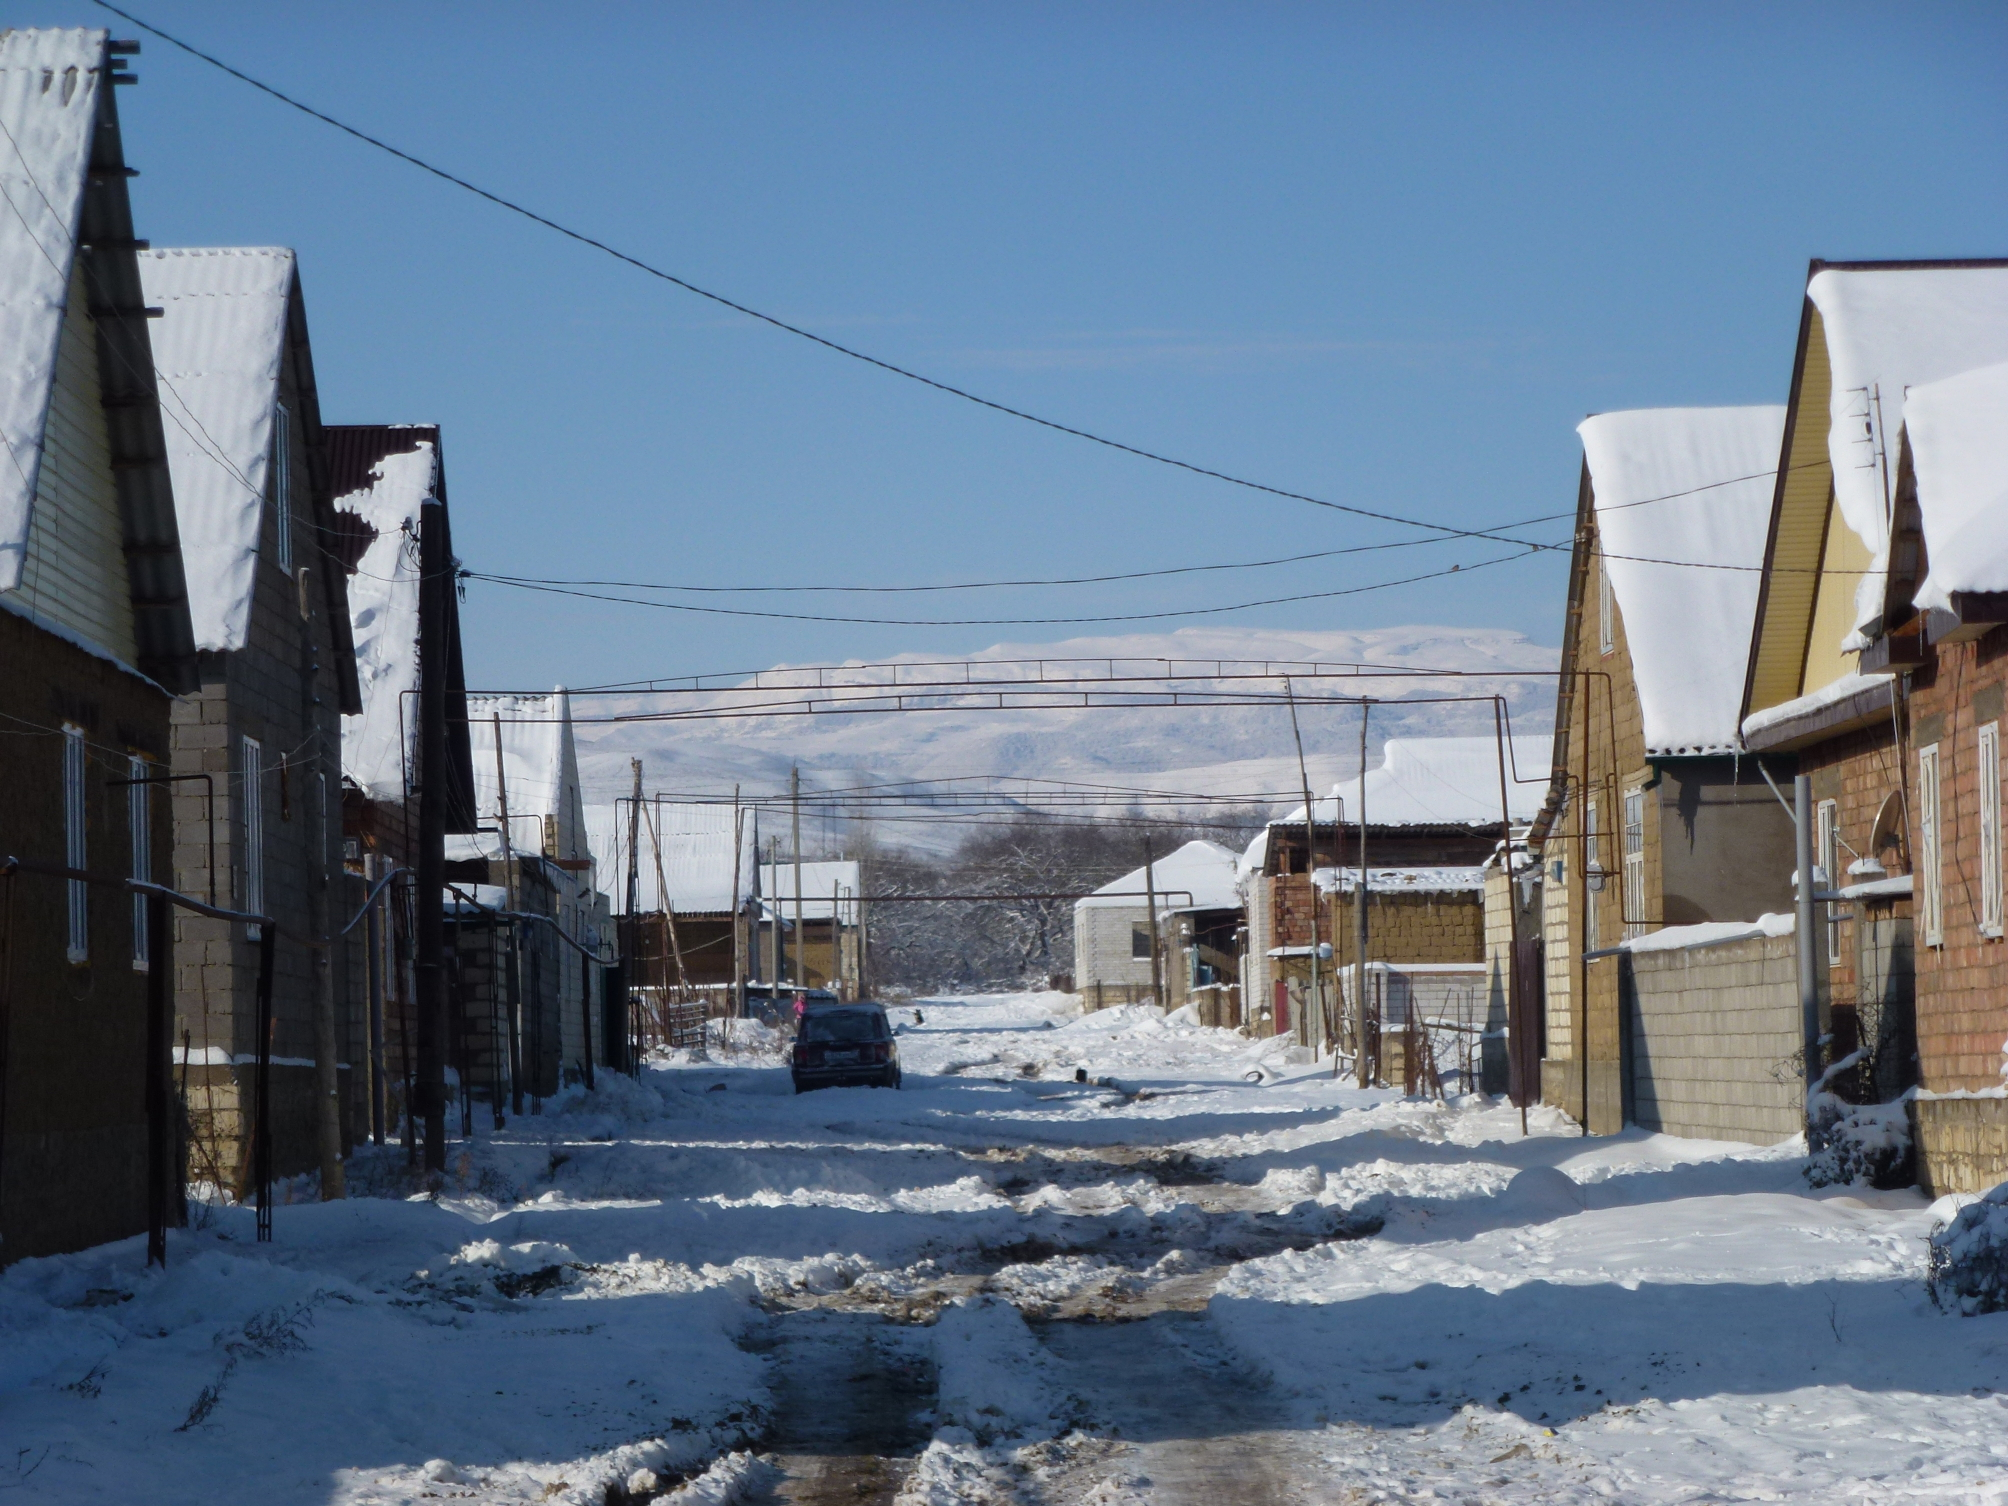
\includegraphics[scale=0.2]{figures/Druzhba.png}
\end{figure}


\begin{figure}[t!]
	\caption{Map of Daghestan}
	\label{fig:Map 2}
	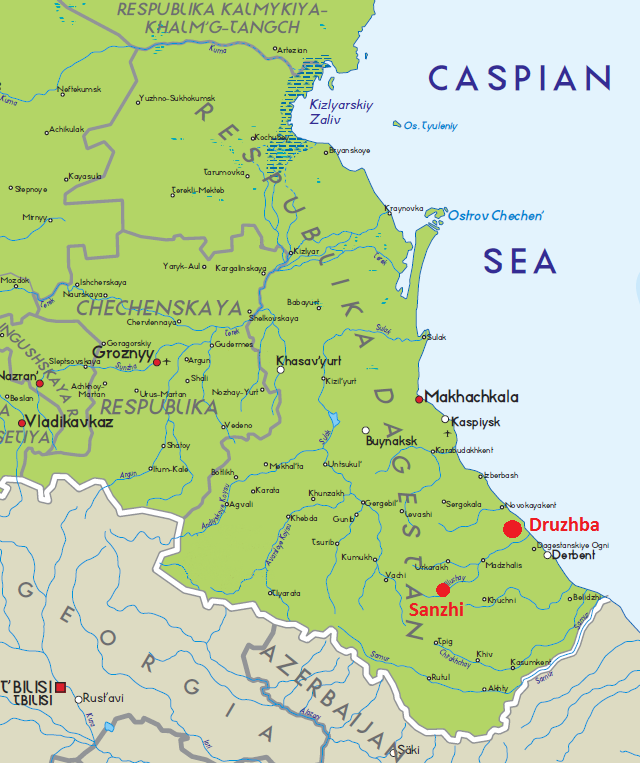
\includegraphics[scale=0.7]{figures/Dagestan_Sanzhi.png}
\end{figure}

%%%%%%%%%%%%%%%%%%%%%%%%%%%%%%%%%%%%%%%%%%%%%%%%%%%%%%%%%%%%%%%%%%%%%%%%%%%%%%%%

\section{The sociolinguistic situation of Sanzhi}
\label{sec:The sociolinguistic situation of Sanzhi}

All languages of the Republic of Dagestan are official languages, but only 14 of them have the status of being officially written languages. Sanzhi Dargwa, like many other comparatively small languages and varieties spoken on the territory of Dagestan, does not belong to the written languages.  

Before the arrival of Russian in the remote parts of the central Dagestanian mountains, where the original village of Sanzhi is located, Kumyk served as the language of interethnic communication in the wider area. The main traces of contact with Kumyk are the numerous Turkic loan words (e.g. the first part in \textit{ač barq'ij} `open' originates from the Kumyk verb \textit{ač-maq}, \textit{baχča} `garden' (identical in Kumyk), \textit{qːʷaz} `goose' from Kumyk \textit{qaz}, and many more). Nevertheless, among the Sanzhi speakers with whom I worked, nobody claimed to have a significant command of Kumyk. All villages, except for one\footnote{The exception is an Agul village.} in the immediate neighborhood of Sanzhi, are Dargwa villages with Dargwa varieties closely related to Sanzhi, so that communication was and still is easily possible just by sticking to one's own variety.

\begin{figure}
	\caption{Sanzhi men at the Uraza Bayram, the holiday at the end of Ramadan in 2013 (Gadzhimurad Gadzhimuradov, who is dressed in dark clothes, is standing on the left side) (picture by Diana Forker)}
	\label{fig:SanzhiPeople}
	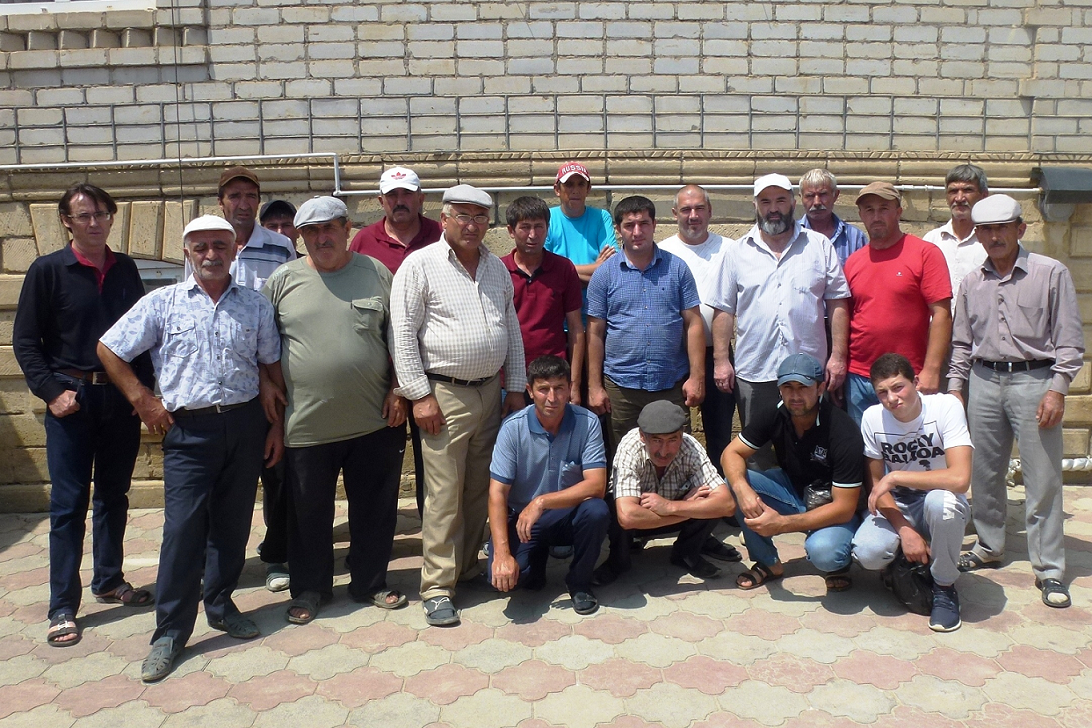
\includegraphics[scale=0.4]{figures/8_uraza2013.png}
\end{figure}

Today, all Sanzhi speakers are bilingual or multilingual to various extents because they know at least some Russian. Russian serves as the main language of interethnic communication and is the only language used in education and administration, and more generally in the public sphere in Dagestan. The degree of bilingualism varies from speaker to speaker, but simplifying somewhat, we can say that women of the oldest generation (60 years and older) are the only group that is dominant in Sanzhi. Men of the oldest generation as well as many members of the middle generation (age 30 to 60) are more or less balanced bilinguals, and use the two languages in accordance with the different functional domains (public/official vs. private/speech community). All members of the youngest generation are dominant in Russian, but everybody has at least a passive command of Sanzhi and is able to use a simplified form of the language in communication with members of the oldest generation, e.g. in interaction between grandchildren and grandparents.

Thus, the contact situation is largely language maintenance for the oldest and middle generation. Among the youngest generation we observe language shift, and we can assume that members of the youngest generation in particular who are still children today will not pass on Sanzhi to their children. Some children and young people in Druzhba still learn Sanzhi as their first language (this depends on the family situation), but they come in contact with Russian right from the first day of their life. Russian becomes the dominant language at the latest when children start attending kindergarten. Therefore, they generally have a limited and mostly passive command of Sanzhi and prefer to speak only Russian. Sanzhi people of the young generation, including small children, speak predominantly Russian with each other. More and more Sanzhi people speak Russian not only to their neighbors in Druzhba, many of which are from other ethnic groups, but even at home. Although the people have a positive language attitude and are proud of speaking their own language, Russian is considered to be not only more prestigious, but extremely necessary for the future of their children (see \citealt{ForkerSubmitteda} for more information).

Another factor influencing the linguistic situation is marriage between women and men from different ethnic groups, which usually does not lead to bilingual children acquiring both the language of the mother and of the father, but to children speaking only Russian at home, as the parents use Russian to communicate with each other. I estimate that there are only a few families left in which both husband and wife are competent Sanzhi speakers that have grown up in the village of Sanzhi. We can assume that in the past the situation must have been different and the vast majority of wives were either from Sanzhi or from the surrounding villages (Itsari, Chakhri, Kunki, Duakar, Dzilebki are the main villages of origins of mothers and wives of the Sanzhi speakers with whom I worked).

Since Sanzhi Dargwa is not employed in the public domain (e.g. administration, education, media,  court) the language is unwritten and used only for oral communication within the Sanzhi community. The only printed material so far is \citet{Forker.Gadzhimuradov2017}, a collection of traditional stories and other texts. In school, Sanzhi children have around two hours of mother tongue education per week, during which they learn Standard Dargwa. Sanzhi speakers do not understand literary Standard Dargwa, because Akusha Dargwa, the base for the standard language, is a Northern Dargwa variety and quite different from Sanzhi. Therefore, in spite of the school classes, Sanzhi children usually do not learn Standard Dargwa well and are not able to speak, write, or read in Standard Dargwa, or make use of the few newspapers and TV programs offered.



%%%%%%%%%%%%%%%%%%%%%%%%%%%%%%%%%%%%%%%%%%%%%%%%%%%%%%%%%%%%%%%%%%%%%%%%%%%%%%%%

\section{Genealogical affiliation}
\label{sec:Genealogical affiliation}

Sanzhi belongs to the Dargwa (Dargi) languages, which form a subgroup of the East Caucasian (Nakh-Daghestanian) language family. The exact number of languages belonging to this family is unknown, but it can be estimated to be around 40. The internal classification of the family has not yet been unanimously resolved. \reffig{fig:classificationtree} shows one of the possible classifications (namely the classification according to \citealt[xi]{Kibrik1996}). The internal division of the Dargwa branch into subvarieties is largely taken from \citet{Korjakov2006}. Dargwa languages are commonly divided into a Northern Dargwa group and a Southern Dargwa group, whereby Sanzhi belongs to the latter. The spelling of the names for languages and varieties in  \reffig{fig:classificationtree} follows the conventions established in the literature and in the recent handbooks on East Caucasian languages \citep{PolinskyInPress, KoryakovEtAllInPreparation}. Unfortunately, in a few cases this leads to differences between the spelling of a village name and the spelling of the language spoken in it (e.g. the village of Itsari vs. Icari Dargwa).
%
\begin{figure}
	\caption{A family tree of East Caucasian}
	\label{fig:classificationtree}

	\small
	\begin{itemize}
		\item[]	Nakh branch
		\item[]	\qquad\tit{Chechen, Ingush, Tsova-Tush (Batsbi)}

		\item[]	Avar-Andic-Tsezic subbranch
		\item[]	\qquad Avar-Andic
		\item[] \qquad\qquad \textit{Avar}
		\item[]	\qquad\qquad Andic
		\item[]	\qquad\qquad\qquad\tit{Andi, Botlikh, Godoberi, Karata, Akhvakh, Bagvalal,} 
		\item[]	\qquad\qquad\qquad\tit{Tindi, Chamalal}

		\item[]	\qquad Tsezic subbranch
		\item[]	\qquad\qquad\tit{Tsez, Hinuq, Khwarshi, Bezhta, Hunzib}

		\item[]	Dargwa subbranch
		\item[]	\qquad\tit{Akusha/Standard Dargwa, Urakhi, Mugi, Tsudakhar, Gapshima-Butri,}
		\item[]	\qquad\tit{Mjurego-Gubden, Kadar, Muiri, Mehweb, Sirkhi, Amukh-Xuduc, Shiri,}
		\item[]	\qquad\tit{Qunqi, Icari, \tbf{Sanzhi}, Chirag, Kajtag, Kubachi-Ashti}

		\item[]	\tit{Lak}
		\item[]	\tit{Khinalug}

		\item[]	Lezgic subbranch
		\item[]	\qquad\tit{Udi, Archi, Lezgian, Agul, Tabasaran, Tsakhur, Rutul, Kryz, Budugh}
	\end{itemize}
\end{figure}


%%%%%%%%%%%%%%%%%%%%%%%%%%%%%%%%%%%%%%%%%%%%%%%%%%%%%%%%%%%%%%%%%%%%%%%%%%%%%%%%

\section{Dargwa languages and the problem of the \dqt{Dargwa ethnicity}}
\label{sec:Dargwa languages and the problem of the Dargwa ethnicity}

Today, all languages spoken in the the Republic of Dagestan have the status of official languages (see the article 11 of the constitution of Dagestan, 2003). This includes Standard Dargwa and Russian, among others. There is a distinction between the so-called ``unwritten'' and the ``written languages'' of Dagestan. The latter are (in addition to Russian), Avar, Agul, Azerbaijani, Kumyk, Lak, Lezgian, Noghay, Rutul, Tabasaran, Tat, Tsakhur, and Chechen. Written languages of Dagestan are, in principle, taught in school and used to some extent in the media (e.g. newspapers, journals). Until 1928, speakers of Dargwa varieties used the Arabic script, but there was no standard orthography. From 1925 onwards, the first newspaper in a Dargwa language was published \citep[15]{Abdullaev1954}. This newspaper, as well as most books and other materials, was published in Akusha Dargwa, the language which was later chosen as the basis for the literary standard Dargwa language. There are several reasons for this choice: Akusha was and still is the Dargwa variety with the most speakers, and the village of Akusha together with the surrounding villages formed an autonomous center (\textit{vol'noe obščestvo}) for a long time. In 1930 at the first Dagestanian conference on orthography, Akusha was appointed to be the basis for the literary standard Dargwa language. In 1928, a Latin alphabet was developed for a number of Dagestanian languages including Dargwa, Avar, Lak, Lezgian, and Tabasaran. In 1938 the policy changed completely, and for all Dagestanian literary languages Cyrillic alphabets were introduced \citep[48\tnd51]{Grenoble2003}. In the following years the Dargwa alphabet underwent several changes.

Dargwa people are officially considered to be one group that shares a common ethnicity, and to speak various dialects of one and the same Dargwa language (see below for the viewpoint of linguistics on this). According to the data of the Russian census from 2010, for instance, about 510\ths000 people consider themselves to be ethnic Dargwa, and thus represent the second biggest ethnic group in Dagestan (after the Avars). The vast majority of them claim to speak Dargwa.

Dargwa languages are spoken in the central part of Dagestan (traditionally in the districts Akushinskiy, Levashinskiy, Dakhadayevskiy, Sergokalinskiy, Kaytagskiy, and also partially in the districts of Gunibskiy, Buynakskiy, Karabudakhkentskiy, and Agulskiy), in a territory with a length of about 100 km and a breadth of about 70 km (\reffig{fig:Map 3}). In the west, this area borders on Lak and Avar territory, in the north and east on Kumyk, and in the south on Tabasaran.


\begin{figure}[t!]
	\caption{The East Caucasian (i.e. Nakh-Daghestanian) language family (map courtesy of Yura Koryakov)}
	\label{fig:Map 3}
	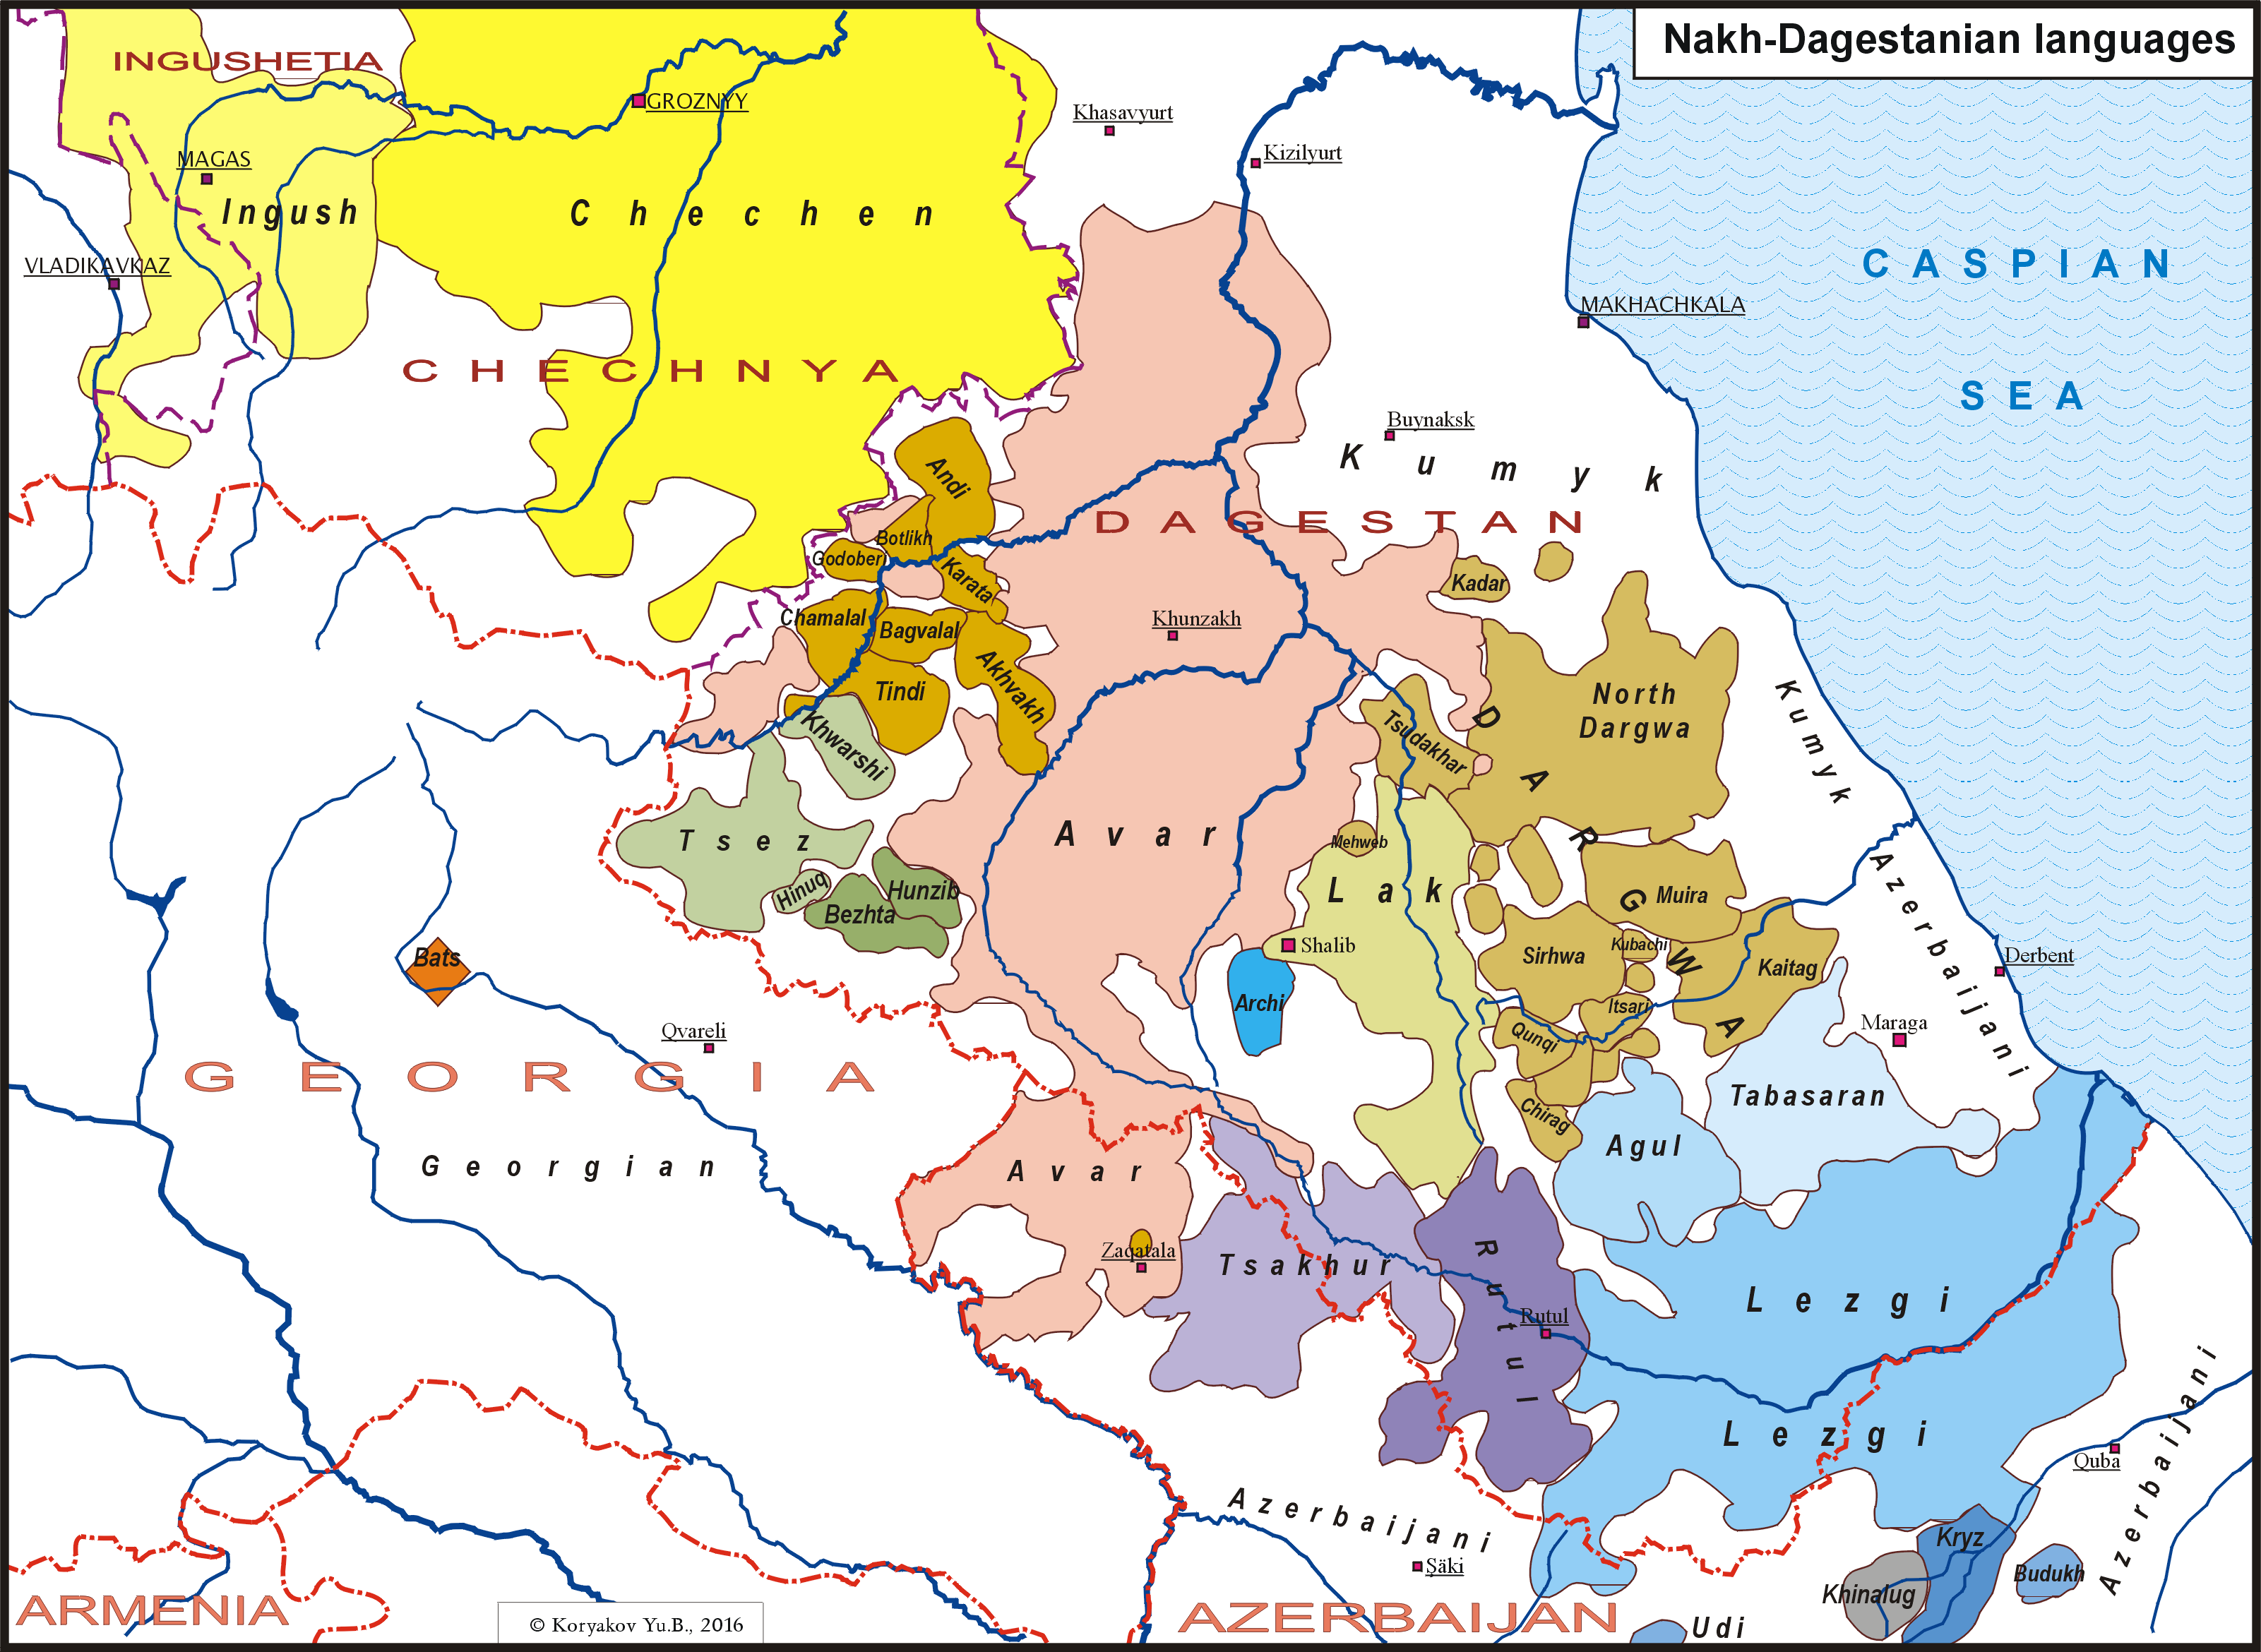
\includegraphics[scale=0.6, angle =90]{figures/NEC_color_2016.png}
\end{figure}

The term \textit{Dargwa} with its current reference was only introduced during Soviet times. There was a policy at the time to create names for peoples and languages that often lacked significance for the people themselves, and to introduce ethnic boundaries all over the Northern Caucasus \citep[114]{Grenoble2003}. The use of these names is nowadays fully established and is largely maintained for political reasons \citep{Shaxbanov2009}.

Historically, the term \textit{Dargwa} (or \textit{Dargi}) does not refer to an ethnic group \citep[13]{Abdullaev1954}. There were seven unions of settlements in central Dagestan that referred to themselves with a proper name and the term \textit{Dargwa}: Akusha-Dargwa, Kaba-Dargwa, Khamur-Dargwa, Bukun-Dargwa, Utsmi (or Kaytag)-Dargwa, Gutsi-Dargwa, and Sirkha-Dargwa \citep[13]{Magomedov1999}. That is, \textit{Dargwa} referred to settlement centers that consisted of a number of small villages forming a unit, which were able to defend themselves and their own interests against enemies (\textit{vol'noe obščestvo}). Other urban centers in the north, like Kadar and Gubden, whose inhabitants are also considered to be Dargwa people today (and to speak Dargwa varieties), did not belong to those units to which the term \textit{Dargwa} was applied. They formed one administrative unit with Kumyk villages \citep[12]{Abdullaev1954}, and used Kumyk as their lingua franca \citep{DobrushinaDanielKoryakov}, \citep[58\tnd59]{Wixman1980}. 

Similarly, there was not one single language with the name \textit{Dargwa}, but a group of related languages, in reference to which the names of the urban centers were used \citep[1]{Uslar1892}. But since Soviet times, the classification of the Dargwa varieties as dialects of one and the same Dargwa language has persisted in many publications and in all official documents (e.g. \citeb{Abdullaev1954}; \citeb{Gasanova1971}; \citeb{Museav2002}; WALS (\url{http://wals.info/}); Ethnologue (\url{http://www.ethnologue.com/})).

Following the most recent publications on the internal classification of the East Caucasian language family \citep{Korjakov2006; Korjakov.Sumbatova2007}, the Dargwa branch consists of 19 languages and about 40 dialects (see \reffig{fig:classificationtree} above). The biggest are Akusha Dargwa (about 42\ths000 speakers), Mjurego-Gubden Dargwa (ca.~39\ths000), Urakhi Dargwa (ca.~35\ths 000), followed by Kajtag Dargwa (ca.~21\ths000), and Tsudakhar Dargwa (ca.~19\ths000). Speakers of most Dargwa languages do not understand each other, and the variation between them is much bigger than between the Andic languages, another subbranch of the East Caucasian family. The break-up of the Proto-Dargwa language can be estimated to have occurred about two millennia ago (Sumbatova, p.c.). However, the exact number of Dargwa languages is still subject to debate, because descriptions are lacking for many of the individual languages and dialects. Thus, \reffig{fig:classificationtree} will likely need to be corrected in the future.

The place of the Dargwa languages inside the East Caucasian family is also debated. Some authors consider them to form a separate branch of the East Caucasian language family \citep[142]{Gigineishvili1977, Kibrik1996}, others group them together with Lak \citep{Haspelmath1993, Korjakov2006, vandenBerg2005}.


%%%%%%%%%%%%%%%%%%%%%%%%%%%%%%%%%%%%%%%%%%%%%%%%%%%%%%%%%%%%%%%%%%%%%%%%%%%%%%%%

\section{Typological overview}
\label{sec:Typological overview}

Sanzhi Dargwa is typologically similar to other East Caucasian languages. It has a relatively large consonant inventory including pharyngeal and ejective consonants, and a medium number of vowels. With respect to its morphosyntactic structure, Sanzhi is predominantly dependent-marking with a rich case inventory. The grammatical cases are ergative, absolutive, dative, and genitive. In addition, there is a plethora of spatial cases. The morphology is concatenative and predominantly suffixing. Sanzhi has an elaborate system of TAM forms. Verbal stems come in pairs that express imperfective and perfective aspect, and many can take spatial preverbs. Salient traits of the grammar are two largely independently operating agreement systems: gender/number agreement and person agreement. Gender/number agreement operates at the phrasal and at the clause level. Within the clause, it is mainly controlled by arguments in the absolutive case and shows up on verbs, adverbs, and on nouns in some of the spatial cases. Person agreement operates at the clausal level only, and functions according to a person hierarchy. Sanzhi has ergative alignment at the level of morphology. SOV is the most frequent constituent order.

Features of Dargwa languages that have attracted the attention of typologists include gender and person agreement \citep{Sumbatova2011, Sumbatova2013, Belyaev2013, Belyaev2017a, Belyaev2017b, GanenkovForthcoming, Forker2016a}, complement constructions including reported speech \citep{Ganenkov2012, ForkerSubmittedb}, experiencer constructions \citep{Comrie.vandenBerg2006, Ganenkov2006, Ganenkov2013}, local and long-distance reflexivization \citep{Forker2014}, backward control and long-distance agreement \citep{Serdobolskaya2009, Serdobolskaya2010, Belyaev2016}, the expression of space \citep{Ganenkov2010, ForkerLTSanzhi}, information structure \citep{Sumbatova2009, Forker.Belyaev2016, Forker2016a}, and the problem of finiteness \citep{Kalinina.Sumbatova2007}.


%%%%%%%%%%%%%%%%%%%%%%%%%%%%%%%%%%%%%%%%%%%%%%%%%%%%%%%%%%%%%%%%%%%%%%%%%%%%%%%%

\section[Literature and previous works]{Literature on Dargwa languages, Dargwa people, and previous works on Sanzhi}
\label{sec:Literature on Dargwa languages, Dargwa people, and previous works on Sanzhi}

In comparison to some other Dagestanian languages, the description of Dargwa languages has a relatively long tradition. However, despite the impressive number of monographs and articles that have been dedicated to various Dargwa languages, the scope and the quality of many of these works cannot satisfy modern scientific standards. Thus, in the following I will mention only those works that are still in use and represent valuable documentations and analyses of Dargwa. For a more detailed overview on the history of the study of Dargwa languages, see \citet{Magometov1983} and also the references in \citet{Temirbulatova2005}.

The first scientific treatment of a Dargwa language (Urakhi) comes from \citet{Uslar1892}, who visited the Caucasus in the second half of the 19th century. The next key scholar is Said Abdullaev, who published a Russian-Dargwa (i.e. Akusha) dictionary and a grammar of Akusha \citep{Abdullaev1950, Abdullaev1954}. Since the 1950s, Gasanova has written many articles and books about various Dargwa languages and dialects, concentrating mainly on Muiri, Mjuregi, Urakhi, and Tsudakhar \citep[e.g.][]{Gasanova1961, Gasanova1971}. Other important scholars are Zapir Abdullaev, who worked on Standard Dargwa and occasionally on Urakhi and Kajtag \citep[e.g.]{Abdullaev1961, Abdullaev1969, Abdullaev1971, Abdullaev1986, Abdullaev1993, AbdullaevEtAl2014}, Musaev, who investigated various Dargwa varieties, including Chirag and Akusha \citep[e.g.][]{Musaev1975, Musaev1978, Musaev1980a, Musaev1980b, Musaev1983, Musaev1984}, works on Sikhi \citep{Kadibagomedov1998}, on Kajtag \citep{Temirbulatova2005} and most notably on Kubachi \citep{Magometov1963}. Recently, two new dictionaries have been published \citep{Jusupov2005, Jusupov2009}. Rasul Mutalov, one of the key participants in the language documentation project resulting in this grammar, has written a number of papers and books on Icari Dargwa and Standard Dargwa \citep{Mutalov1992, Mutalov2002, Mutalov2018}.

In \citey{vandenBerg1999}, the first book in English on a Dargwa language (Akusha), written by \citea{vandenBerg1999} was published, followed by a descriptive grammar of Icari Dargwa, which was co-authored by Nina Sumbatova and Rasul Mutalov \citep{Sumbatova.Mutalov2003}. Icari Dargwa is closely related to Sanzhi Dargwa; the two varieties are mutually intelligible and the Icari grammar was a fruitful source of inspiration for this grammar of Sanzhi.

In Moscow, a group of linguists works on a number of Dargwa languages, of which the major results are comprehensive studies of Tanti \citep{Sumbatova.Lander2014}, Shiri \citep{BelyaevInPreparation}, Mehweb \citep{DanielMehweb}, Ashti \citep{Belyaev2012} and Chirag \citep{GanenkovChirag}. Other important works from the same group are \citet{Kalinina.Sumbatova2007}, \citet{Sumbatova2009, Sumbatova2010, Sumbatova2011, Sumbatova2013}, \citet{Lander2008, Lander2010}, and \citet{Serdobolskaya2009, Serdobolskaya2010}. \citet{SumbatovaInPreparation} provides a recent overview on Dargwa varieties. Sketch grammars in preparation include \citet{GanenkovChiragSketch} and \citet{ForkerSanzhiSketch}.

Topics in the morphosyntax of Sanzhi and other aspects of Sanzhi have been treated in \citet{Forker2016a, Forker2014, Forker2019, ForkerSubmitteda, ForkerSubmittedb, ForkerSubmittedc}. A collection of texts with Russian translations and a Sanzhi-Russian and Russian-Sanzhi dictionary is \citet{Forker.Gadzhimuradov2017}.

With respect to the ethnographic literature on Dargwa people, there is not much to say. There are only two older monographs \citep{Schilling1949, Gadzieva.etal1967}.


%%%%%%%%%%%%%%%%%%%%%%%%%%%%%%%%%%%%%%%%%%%%%%%%%%%%%%%%%%%%%%%%%%%%%%%%%%%%%%%%

\section{Documenting and describing Sanzhi Dargwa}
\label{sec:Documenting and describing Sanzhi Dargwa}

This grammar is the result of a language documentation project, \tit{Documenting Dargi languages in Dagestan \tnd\ Shiri and Sanzhi}, funded by the DoBeS program of the Volkswagen Foundation. The project officially started in 2012 and ran until 2019. Within this project, three linguists (Diana Forker, Rasul Mutalov, Oleg Belyaev), one anthropologist (Iwona Kaliszewska), and student assistants from the University of Bamberg documented, described, and analyzed the two endangered East Caucasian languages Shiri Dargwa and Sanzhi Dargwa.

\sloppy Detailed information about the project, the languages and many texts, recordings and pictures can be found on the project website (\url{http://www.kaukaz.net/dargwa/sanzhi/lexicon/index.htm}). All materials gathered in the project are accessible upon request via the Language Archive hosted by the MPI Nijmegen (\url{http://dobes.mpi.nl/projects/shiri_sanzhi/}). In addition to the grammar of Sanzhi, the major results of the project are a book with narratives, legends and other texts for the Sanzhi community \citep{Forker.Gadzhimuradov2017}, the electronic corpus of Sanzhi texts with audio recordings for every text and many video recordings (around 24 hours of natural speech), and an electronic dictionary. Around 15 hours of speech have been transcribed in ELAN and translated into Russian, and are deposited in the Language Archive (\url{https://archive.mpi.nl/}). A subcorpus of around 10 hours, which amounts to more than 46\ths000 word tokens, has been fully glossed with FLEx (\url{https://software.sil.org/fieldworks/}) and translated into Russian and English. The texts have almost exclusively been recorded by myself in the village of Druzhba. During the recordings I was accompanied by Rasul Mutalov, my fellow project member, linguist and native speaker of the neighboring Icari dialect, or by Gadzhimuard Gadzhimuradov, my main language assistant, who led the conversation and explained the aims of the project to the Sanzhi speakers. After recording the text were transcribed in ELAN by using a Cyrillic orthography (page xvii) and by making use of the help of native speakers. They also provided a Russian translation. In the ELAN file I added a Latin transliteration following the orthography, which is also employed in this grammar (page xvii). From the transcribed texts I chose a subcorpus, transferred the Latin transcription into FLEx, glossed it and partially added English translations to the Russian translations.

The glossed corpus has been put on the internet and is freely is accessible (\url{http://web-corpora.net/SanzhiDargwaCorpus/search/index.php?interface_language=en}). This corpus consists of 75 texts from 24 speakers of Sanzhi who were between 21 and 80 years old when the texts were recorded (mostly between 2012 and 2015). Only three of the speakers were 35 years or younger, whereas most were older than 50. Slightly more than half of the speakers were female, but the majority of texts originate from male speakers. 

The corpus contains the following types of texts:

\begin{itemize}
	\item 32 fairy tales, legends, anecdotes
	\item 8 fairy tales translated from Standard Dargwa and Russian
	\item 10 autobiographical narrations and texts about the history of the village
	\item 4 recipes and other instructions or procedural texts
	\item 3 poems
	\item 3 natural conversations
	\item 11 descriptions, conversations and narratives from the \textit{\textit{Family Problems Picture Task}} \citep{SanRoqueEtAl2012} (additionally archived with PARDISEC, in the collection SocCog, \url{http://catalog.paradisec.org.au/collections/SocCog})
	\item 4 narrations produced by means of stimuli (two ``Pear Stories'', two stories ``Frog, where are you?'') 
\end{itemize}

The natural data has been complemented by many hours of elicitation. All natural examples originating from the corpus are not further marked in this grammar. All examples which have been elicited are marked by (E).

% https://corpus1.mpi.nl/ds/asv/;jsessionid=2E07D70EB3228292714D678A5572555D?0&openpath=node:1615060

\sloppy The electronic dictionary of Sanzhi was built up with Lexique Pro (\url{http://www.lexiquepro.com/}) and has been published with \textit{Dictionaria} \url{https://dictionaria.clld.org/contributions}. The dictionary contains around than 5\ths500 entries written with Cyrillic and Latin script, Russian and English translations, grammatical information, and example sentences as well as audio recordings for (almost) every entry. The dictionary is also accessible via the project homepage (\url{http://www.kaukaz.net/dargwa/sanzhi/lexicon/index.htm}).

In August 2017, my main assistant Gadzhimurad Gadzhimuradov and I were able to print a book with community materials and present it to the Sanzhi community in Druzhba (\reffig{fig:SanzhiBook}). The book contains 42 texts of various genres taken from the corpus (fairy tales, legends, anecdotes, descriptions of games and recipes, oral history, and a poem) written in the Cyrillic Sanzhi script with a sentence-by-sentence translation in Russian, as well as a Sanzhi-Russian and a simplified Russian-Sanzhi dictionary, which is also available on the project website.

Within the project I have undertaken more than ten field trips to Druzhba (including two short trips to Sanzhi in 2013 and 2016) in order to gather materials on the language. My major language assistant and consultant during all these years was and is Gadzhimurad Gadzhimuradov (\reffig{fig:SanzhiPeople}), a videographer and cameraman from Druzhba, who was born in Sanzhi. After spending his first five years there, his family moved to Druzhba, but he has ever since kept close relationships with the village and is a strong patriot in the best sense. Without the support and friendship of him and his family, in particular his wife Batichay, neither the grammar nor the entire project could have been realized. Gadzhimurad Gadzhimuradov not only helped me to gather, transcribe, and translate materials, he also made many recordings by himself, translated texts into Sanzhi and raised the interest of the Sanzhi community in the project. Patiently he sat down endless hours with me to go through morphological and syntactic paradigms. This grammar could not have been written without his assistance.



\begin{figure}
	\caption{Gadzhimurad Gadzhimuradov presenting the first book in Sanzhi (courtesy of Gadzhimurad Gadzhimuradov, 2017)}
	\label{fig:SanzhiBook}
	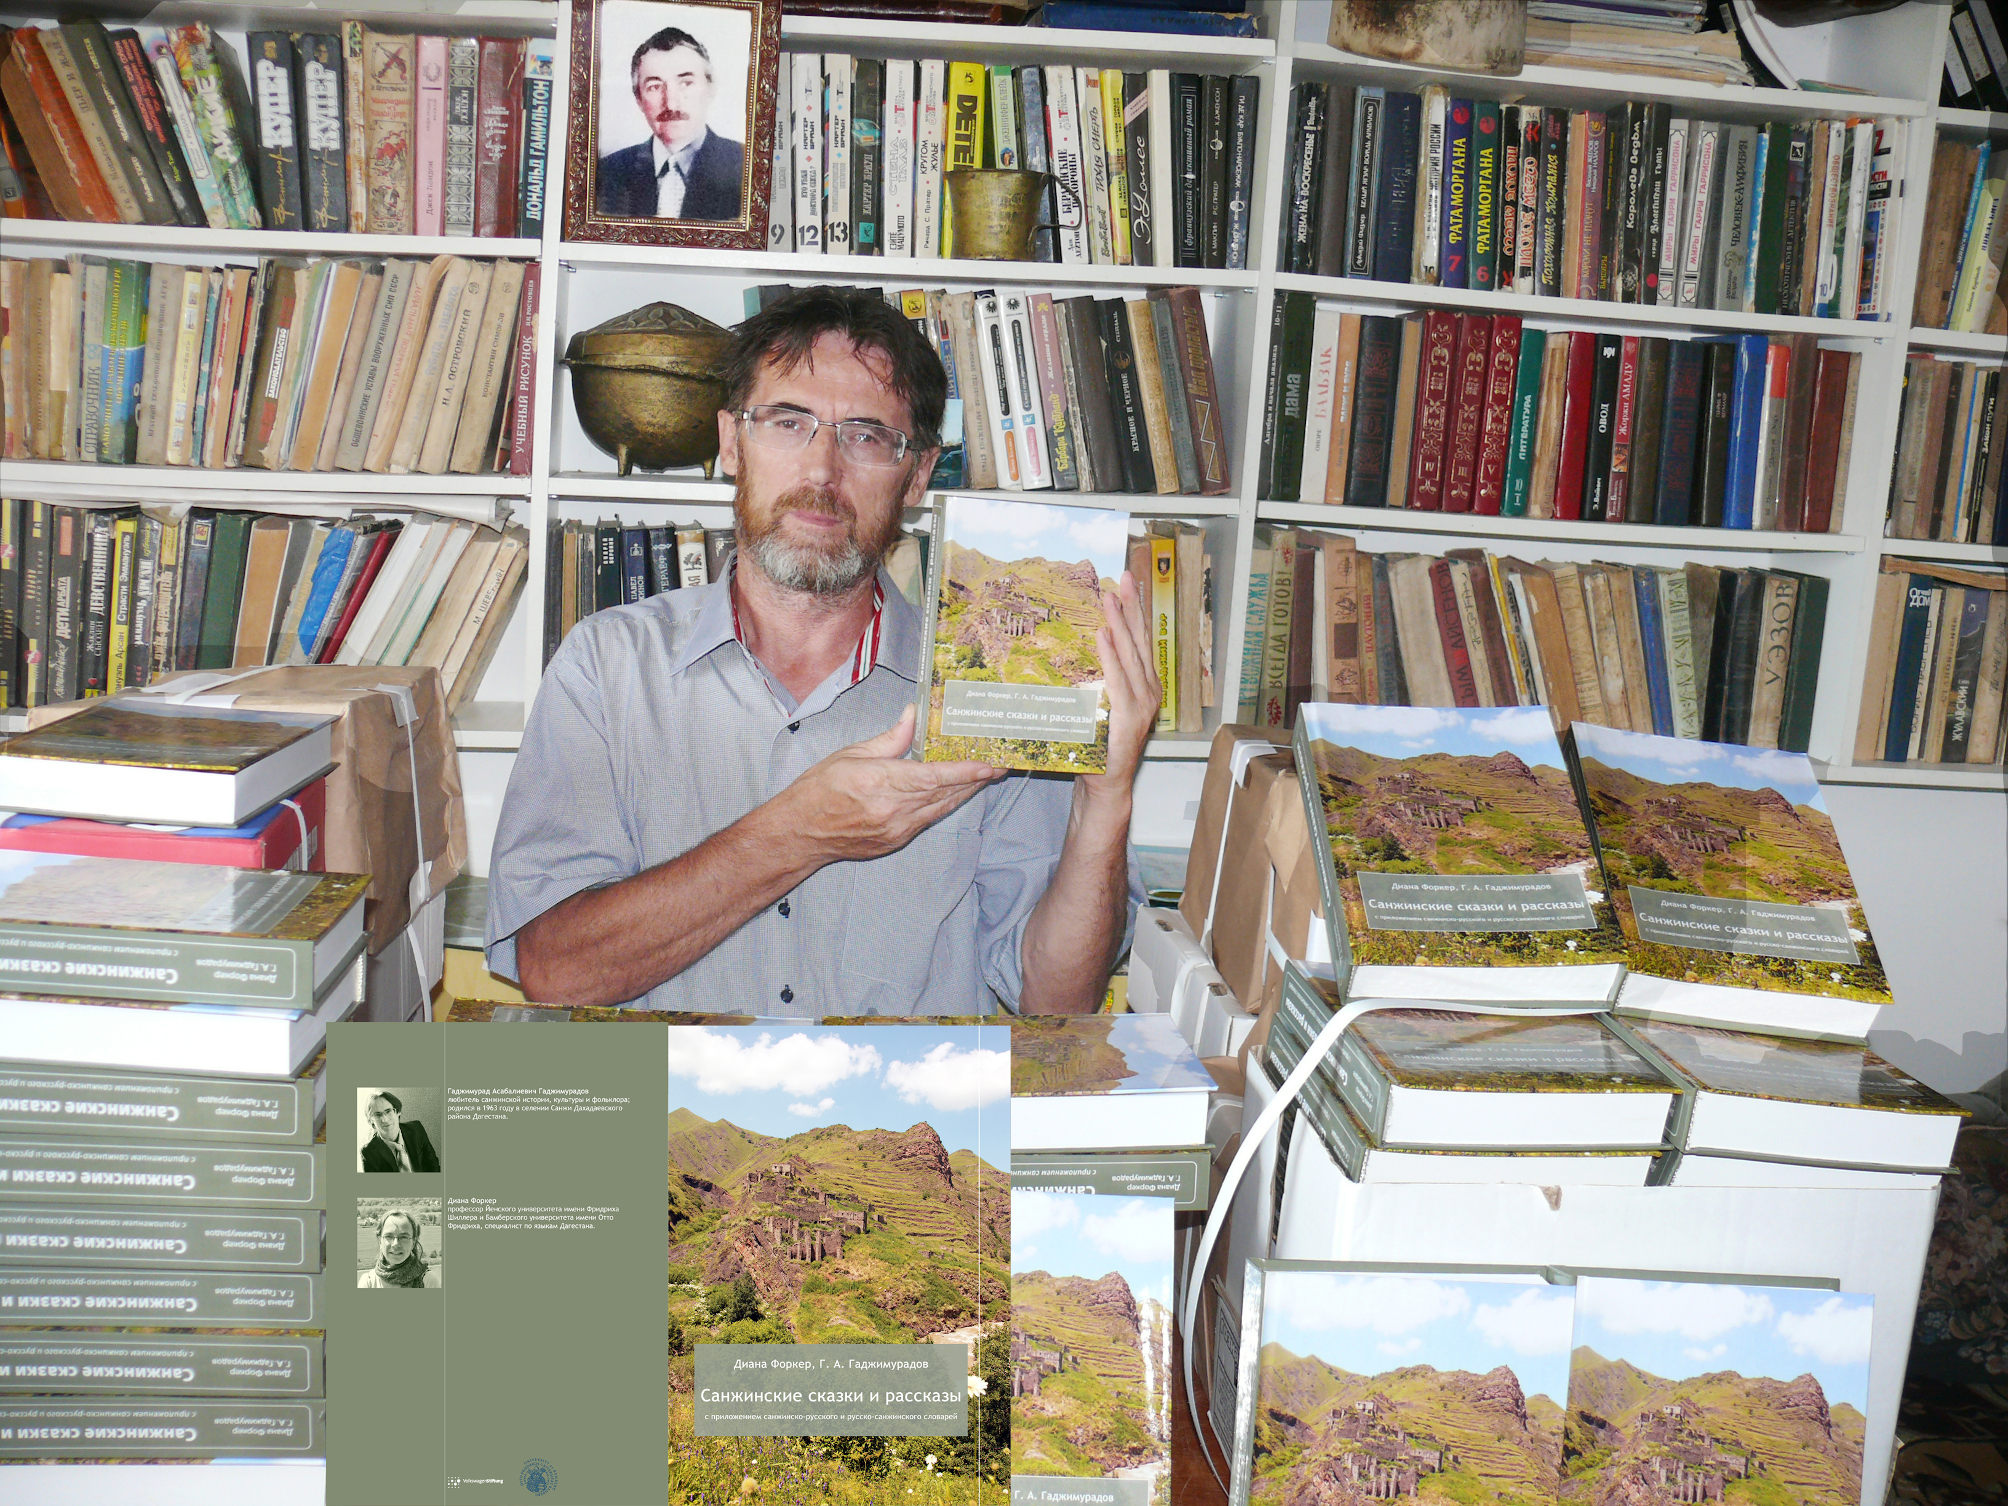
\includegraphics[scale=0.1]{figures/SanzhiBooks1.png}
\end{figure}
